\chapter{Conceptual study}
\label{chap:conceptual}

The deciding factor for the success of one application and the failure of another is the architecture.
In order to achieve the requirements we set in the previous chapter, along with solving the issues faced by the existing solutions, we need to carefully design our systems.

In this chapter, we will first dive into the realm of real-time collaboration and read into the existing theoretical research in the field and its practical applications in the real world.
Then, we will explore the different architectures for building and scaling our application. Finally, we will present the sequence and class diagrams to better define the implementation of our ideas and the trajectory of our work in the following chapter.

\section{Real-time collaboration}

Real-time collaboration is a type of collaboration used in editors and web applications with the goal of enabling multiple users on different computers or mobile devices to modify the same document with automatic and nearly instantaneous merging of their edits.
The document could either be a computer file, stored locally, or a cloud-stored data shared over the internet, such as an online spreadsheet, a word processing document, a database, or a presentation.

Multiple web applications support real-time collaboration under various names.
Microsoft, for example, refers to it as "co-authoring" and offers it as part of its Microsoft Office bundle, including Word, Excel, and PowerPoint~\autocite{noauthor_document_nodate}.
Google Docs is another notorious contender in the space of collaborative editing, with products such as Google Docs and Google Sheets.

The interest in collaborative software has seen a resurgence since 2020, mainly due to the move to remote work, with companies like Microsoft offering ready-to-use APIs to enable this feature.

Real-time collaboration is different from other offline or delayed collaborative approaches, such as Git.
While real-time editing performs automatic, frequent, or even instantaneous synchronization of data between all the connected users, offline editing requires manual submission, merging, and resolution of editing conflicts.

\subsection{History}

In 1968, Douglas Engelbart introduced the first collaborative real-time editor in a presentation named "The Mother of All Demos", which also demonstrated many other fundamental elements of modern personal computing including windows, hypertext, graphics, video conferencing, the computer mouse, word processing, and revision control~\autocite{noauthor_firsts:_nodate}.

It took many decades for collaborative software to become mainstream.
One of the first editors that offered collaborative capabilities was Writely, a collaborative word processor launched in 2005~\autocite{chang_ehub_2005}.
It was later acquired by Google and renamed to Google Docs~\autocite{noauthor_google_2006}.
Another Google-backed product from the same era was Google Wave, a collaborative email software. However, less than a year later, it was discontinued due to a lack of users~\autocite{fried_google_nodate}.

Since 2010, the number of web-based collaborative software has been exploding with successful examples such as Figma and Notion. Figure~\ref{fig:timeline-collab} shows the resurgence of products with real-time collaboration.

\begin{figure}
	\centerfloat
	\startchronology[startyear=1960, height=0.1pc, arrow=false]
	\chronoevent{1968}{"The Mother of All Demos" \endgraf by Douglas Engelbart}
	\chronoevent[markdepth=56pt]{2006}{Writely}
	\chronoevent{2009}{Google Wave}
	\chronoevent[markdepth=104pt]{2016}{Notion}
	\chronoevent[markdepth=64pt]{2016}{Figma}
	\chronoevent[markdepth=24pt]{2018}{Notion 2}
	\stopchronology

	\caption{Timeline of real-time collaboration}
	\label{fig:timeline-collab}
\end{figure}

\subsection{Theoretical grounds}

The main challenge of real-time collaboration is keeping multiple clients in sync.
An algorithm has to be employed to determine how to apply---often conflicting---edits from the different remote users.
Network latency is the main culprit for such a dilemma as modifications can reach the other clients with a certain amount of delay.
Figure \ref{fig:collab-problem} shows a common example of conflicting changes by two users caused mainly by network latency.

\begin{figure}[H]
	\centerfloat
	\begin{tikzpicture}[node distance=2.0cm]

		\node(original) {Mary};
		\node(alice-1)[below left of=original] {M\textcolor{red}{\cancel{ar}}y};
		\node(alice-2)[below of=alice-1] {My};
		\node(bob-1)[below right of=original] {\textcolor{red}{\cancel{M}}\textcolor{green}{H}ary};
		\node(bob-2)[below of=bob-1] {Hary};
		\node(result)[below right of=alice-2] {?};

		\node[right of=bob-1] {Bob};
		\node[left of=alice-1] {Alice};

		\draw[->] (original) -- (alice-1) -- (alice-2) -- (result);
		\draw[->] (original) -- (bob-1) -- (bob-2) -- (result);
	\end{tikzpicture}

	\caption{Example of a common problem in real-time collaboration}
	\label{fig:collab-problem}
\end{figure}

Over the years, two main algorithms emerged for dealing with real-time collaboration, \acrfull{crdt} and \acrfull{ot}.
Both have their benefits and drawbacks, and each one has numerous variations and implementations.

\subsubsection{\acrfull{ot}}

\acrlong{ot} was invented for supporting real-time co-editors in the late 1980s and has evolved to become a collection of core techniques widely used in today's working co-editors and adopted in major industrial products~\autocite{sun_real_2020}.
Google Docs has been using \acrshort{ot} since at least 2009~\autocite{noauthor_whats_nodate}.

The model of \acrlong{ot} works by calculating all possible transformations for a text and using them to transform received changes according to the local state, thus eliminating any possible mistakes of synchronization.
Figures~\ref{fig:ot-sol-before} and~\ref{fig:ot-sol-after} explain the algorithm followed by \acrshort{ot} for resolving conflicts.
Figure~\ref{fig:collab-sol-ot} illustrates the solution proposed by \acrshort{ot} for the problem proposed in~\ref{fig:collab-problem}.


\begin{figure}[H]
	\centerfloat
	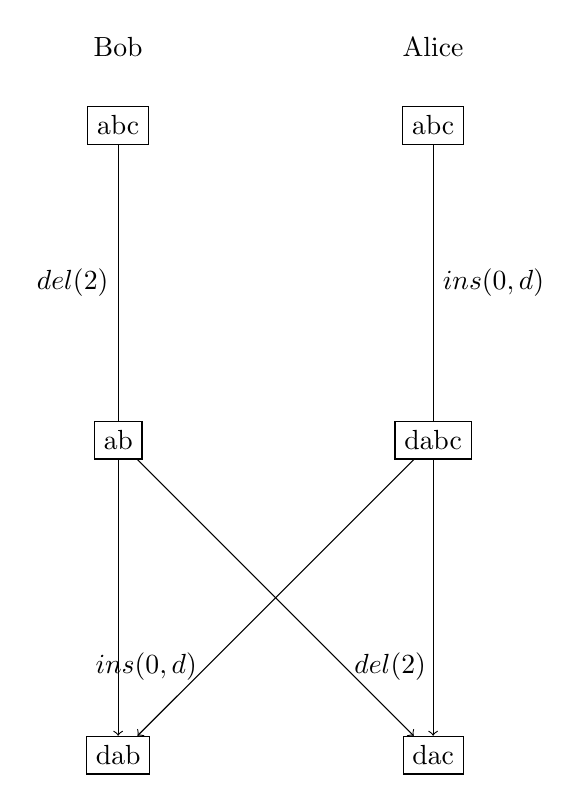
\begin{tikzpicture}[node distance=4cm]

		\node(bob-1)[rectangle, draw=black] {abc};
		\node(bob-2)[rectangle, draw=black, below of=bob-1] {ab};
		\node(bob-3)[rectangle, draw=black, below of=bob-2] {dab};

		\node(alice-1)[rectangle, draw=black, right of=bob-1] {abc};
		\node(alice-2)[rectangle, draw=black, below of=alice-1] {dabc};
		\node(alice-3)[rectangle, draw=black, right of=bob-3] {dac};

		\node at (0,1) {Bob};
		\node at (4,1) {Alice};


		\draw[->] (bob-1) --node[left]{$del(2)$} (bob-2) -- (bob-3);
		\draw[->] (alice-1) --node[right]{$ins(0,d)$} (alice-2) -- (alice-3);
		\draw[->] (alice-2) --node[left, near end]{$ins(0,d)$} (bob-3);
		\draw[->] (bob-2) --node[right,near end]{$del(2)$} (alice-3);
	\end{tikzpicture}
	\caption{Without \acrshort{ot}}
	\label{fig:ot-sol-before}
\end{figure}

\begin{figure}[H]
	\centerfloat
	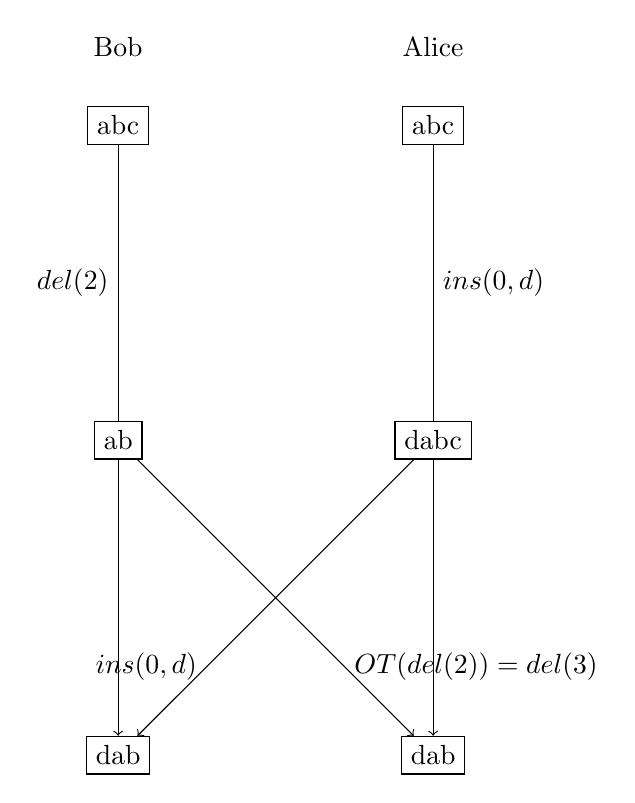
\begin{tikzpicture}[node distance=4cm]

		\node(bob-1)[rectangle, draw=black] {abc};
		\node(bob-2)[rectangle, draw=black, below of=bob-1] {ab};
		\node(bob-3)[rectangle, draw=black, below of=bob-2] {dab};

		\node(alice-1)[rectangle, draw=black, right of=bob-1] {abc};
		\node(alice-2)[rectangle, draw=black, below of=alice-1] {dabc};
		\node(alice-3)[rectangle, draw=black, right of=bob-3] {dab};

		\node at (0,1) {Bob};
		\node at (4,1) {Alice};


		\draw[->] (bob-1) --node[left]{$del(2)$} (bob-2) -- (bob-3);
		\draw[->] (alice-1) --node[right]{$ins(0,d)$} (alice-2) -- (alice-3);
		\draw[->] (alice-2) --node[left, near end]{$ins(0,d)$} (bob-3);
		\draw[->] (bob-2) --node[right,near end]{$OT(del(2))=del(3)$} (alice-3);
	\end{tikzpicture}
	\caption{With \acrshort{ot}}
	\label{fig:ot-sol-after}
\end{figure}


\begin{figure}[H]
	\centerfloat
	\begin{tikzpicture}[node distance=2.0cm]

		\node(original) {Mary};
		\node(alice-1)[below left of=original] {M\textcolor{red}{\cancel{ar}}y};
		\node(alice-2)[below of=alice-1] {My};
		\node(alice-3)[below of=alice-2] {Hy};
		\node(bob-1)[below right of=original] {\textcolor{red}{\cancel{M}}\textcolor{green}{H}ary};
		\node(bob-2)[below of=bob-1] {Hary};
		\node(bob-3)[below of=bob-2] {Hy};

		\node[right of=bob-1] {Bob};
		\node[left of=alice-1] {Alice};

		\draw[->] (original) -- (alice-1) -- (alice-2) -- (alice-3);
		\draw[->] (original) -- (bob-1) -- (bob-2) -- (bob-3);
		\draw[->] (bob-2) --node[below]{\textcolor{red}{\cancel{M}}\textcolor{green}{H}} (alice-2);
		\draw[->] (alice-3) --node[below]{\textcolor{red}{\cancel{ar}}} (bob-2);
	\end{tikzpicture}

	\caption{\acrshort{ot}'s solution for the problem in figure~\ref{fig:collab-problem}}
	\label{fig:collab-sol-ot}
\end{figure}

As seen in the previous examples, \acrshort{ot} can be hard and costly to set up, even for text-based documents.
When it comes to more complicated and nested data structures, \acrshort{ot} is rarely the first choice.

\subsubsection{\acrshort{crdt}}

\acrlong{crdt} is a data structure that was first proposed around 2006 under the name of \acrfull{woot}~\autocite{sun_real_2020}.
It has the benefit of being able to be duplicated over numerous computers in a network, where the replicas can be updated independently and concurrently without requiring coordination, and where inconsistencies can always be resolved mathematically~\autocite{shapiro_conflict-free_2011}.

In 2011, \acrshort{crdt} was formally defined~\autocite{shapiro_conflict-free_2011}, and while it was initially developed for collaborative text editing, it was eventually adopted for multiple other use cases such as online chat systems and distributed databases.

\acrshort{crdt} is further subdivided into two types based on its implementation---\acrfull{cmrdt} and \acrfull{cvrdt}. Both of them offer the same real-time capabilities but differ in their design and approach to the concept.

\paragraph{\acrshort{cmrdt}}

\acrlong{cmrdt} or Operation-based \acrshort{crdt} transmits the local state only by sending the update operations required to reach that state.
Upon receiving these operations, remote clients must apply them to become in sync with the sender. The transmission server has to avoid duplicating the operations as this algorithm is not idempotent.

\paragraph{\acrshort{cvrdt}}

\acrlong{cvrdt} or State-based \acrshort{crdt} sends over the whole local state to be merged with the receiving clients' states. This method tends to be slow due to the need of sending large amounts of data instantaneously over the network. However, the infrastructure does not have to deal with deduplication as it is the case with \acrshort{cmrdt}s.

\subsection{Practical examples}

In practice, web applications do not adhere to one algorithm. Instead, they draw from different concepts to a solution that perfectly fits their needs.

\subsubsection{Figma}

Figma is one of the first web design tools with real-time collaboration.
It was released in 2016 and since then it has been hailed as one of the best examples of performant and collaborative software.


% refer to ther blog post

\subsubsection{Excalidraw}
Excalidraw is an open-source white-board and wireframing web application.

% refer to their blog post
\subsubsection{Automerge}

Automerge is a JavaScript data structure designed specifically for collaborative software.

% refer to their github

\subsubsection{Centige}

Centige is a discontinued collaborative web app builder by the author.
It was mainly a learning project, started in late 2019 and developed throughout 2020.

% explain your experience

\subsection{Conclusion}
% What the current choice: we're using blocks -> easy collaboration

\section{Design patterns}
\subsection{Common patterns}
\subsection{Comparison}
\subsection{Conclusion}

\section{Detailed architecture}
\section{Class diagrams}
\section{Sequence diagrams}
\section{Activity diagrams}

\section{Conclusion}